%&"../ai"
\endofdump  % Starts the dynamic preamble
\tikzexternalize[prefix=cache/]{hw01}  % Obvious definition on the jobname is required.
\begin{document}

    \title{第一次作业}
    \maketitle

    \begin{problem}
        比较宽度优先算法(BFS)、一致代价搜索(UCS)、深度优先算法(DFS)的优劣。
    \end{problem}

    \begin{solution}
        优劣比较如下表所示。
        \begin{table}[H]
            \centering
            \begin{tabular}{>{\bfseries}cp{7cm}p{7cm}}
                \toprule
                    & \bfseries\hfil 优势 \hfil & \bfseries\hfil 劣势 \hfil \\
                \midrule
                BFS & 时间复杂度对于较浅解较好$O(b^{d})$ & 空间复杂度大$O(b^d)$ \\
                UCS & 能够查找任何耗散函数$g$,而不仅仅是深度上的比较 & 最坏情况下时空复杂度大$O(b^{1+\lfloor C^\ast/\epsilon \rfloor})$,需要每步代价$\epsilon\geq 0$      \\
                DFS & 空间复杂度较小$O(bm)$      & 不具有完备性和最优性      \\
                \bottomrule
            \end{tabular}
            \begin{quotation}
                \footnotesize $b$指分支因子,$d$指最浅解的深度,$m$指搜索树最大深度。$C^\ast$为最优解的代价,假设每个行动的代价至少为$\epsilon$。
            \end{quotation}
        \end{table}
    \end{solution}

    \begin{problem}
        说明有信息搜索与无信息搜索的区别。
    \end{problem}

    \begin{solution}
        \textbf{有信息搜索}需要访问启发式函数$h(n)$来估算从$n$到目标的解代价,并由此来选择扩展节点---相比其他状态“更有希望”接近目标。而\textbf{无信息搜索}除了问题定义中提供的状态信息外没有任何附加信息,更加盲目,不做这种估计并相对局部地进行搜索判断。
    \end{solution}

    \begin{problem}
        假如我们现在有一个长度为$M$个格子、宽度为$N$个格子的棋盘,盘子中有一些障碍物、形成了一个迷宫。有两个机器人希望根据他们的位置让他们尽快相遇(相遇指的是让两个机器人处在同一个格子里即可,不需要让他们面对面朝向)。机器人在一个行动单位内可以沿着自己朝向的方向移动到一个相邻的格子内、或者旋转自己朝向的方向$90^{\circ}$。
        \begin{enumerate}
            \item 请将该问题形式化,我们需要如何简单地定义该问题的状态(state)?
            \item 对于该状态而言,你定义的状态其状态空间有多大(size)?
            \item 继续形式化该问题,描述该问题的行动、目标测试、路径耗散(简单描述即可)。
            \item 如果使用搜索算法解决该问题,请给出一个启发函数$h$,该启发函数满足可接受性。
        \end{enumerate}
    \end{problem}

    \begin{solution}
        \begin{enumerate}
            \item 两个机器人所处的位置、朝向。
            \item 由于每个机器人的朝向可以有4个,所以状态空间的大小为
            \begin{equation*}
                (4^{MN})^2=16^{MN}
            \end{equation*}
            但是棋盘中可能会有障碍物,所以状态空间大小会小于等于上面的值。更确切地说,如果棋盘中有$p$个无障碍物位置,则状态空间的大小就是
            \begin{equation*}
                16^p \quad (p\leq MN)
            \end{equation*}
            \item 
            \begin{description}
                \item[行动] 机器人旋转朝向$90^\circ$,或在前方无障碍物的情况下沿自己朝向前进一格。
                \item[目标测试] 两个机器人是否处在同一个格子内。
                \item[路径耗散] 以一个简单的$2\times 2$棋盘为例,将每个可行位置分为4种状态,单向连接可通过对应朝向到达的状态对,并双向连接单个格子内每个相邻转向状态。
                \begin{figure}[H]
                    \centering
                    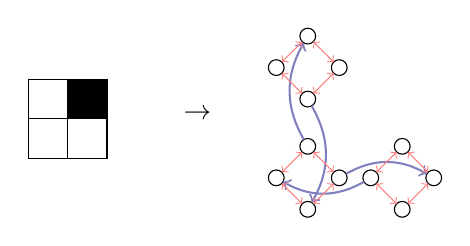
\begin{tikzpicture}
      \tikzstyle{bordered} = [draw,outer sep=0,inner sep=1,minimum size=0.5cm]
      \tikzstyle{state} = [draw,circle,outer sep=0,inner sep=1,minimum size=0.2cm]
      \tikzstyle{move}=[->,bend left,line width=0.75pt,blue!50!black!50]
      \tikzstyle{turn}=[<->,red!50]
	\node [bordered] at (-0.5,0) {};
\node [bordered,fill] at (0,0) {};
\node [bordered] at (-0.5,-0.5) {};
\node [bordered] at (0,-0.5) {};
\node [state] (v9) at (2.4,0.4) {};
\node [state] (v4) at (2.8,0.8) {};
\node [state] (v10) at (3.2,0.4) {};
\node [state] (v1) at (2.8,0) {};
\node [state] (v3) at (2.8,-0.6) {};
\node [state] (v8) at (2.4,-1) {};
\node [state] (v2) at (2.8,-1.4) {};
\node [state] (v5) at (3.2,-1) {};
\node [state] (v7) at (3.6,-1) {};
\node [state] (v11) at (4,-0.6) {};
\node [state] (v6) at (4.4,-1) {};
\node [state] (v12) at (4,-1.4) {};
\draw [move] (v1) edge (v2);
\draw [move] (v3) edge (v4);
\draw [move] (v5) edge (v6);
\draw [move] (v7) edge (v8);
\draw [turn] (v4) edge (v9);
\draw [turn] (v9) edge (v1);
\draw [turn] (v1) edge (v10);
\draw [turn] (v10) edge (v4);
\draw [turn] (v3) edge (v8);
\draw [turn] (v8) edge (v2);
\draw [turn] (v2) edge (v5);
\draw [turn] (v5) edge (v3);
\draw [turn] (v7) edge (v11);
\draw [turn] (v11) edge (v6);
\draw [turn] (v12) edge (v6);
\draw [turn] (v12) edge (v7);
\node at (1.4,-0.2) {$\rightarrow$};
\end{tikzpicture}
                \end{figure} 
                而路径耗散就是对这个转换后的状态图上的每一条边设置一个1的权值。
            \end{description}
            \item 启发函数$h$被定义为两个机器人之间的曼哈顿距离。这个函数满足可接受性,因为机器人不能斜着走,中间有障碍会导致其行动比这个距离长,而且还需要考虑转向也会需要更多的路径耗散。
        \end{enumerate}
    \end{solution}

    \begin{problem}
        证明以下结论(仅需要简单说明证明思路即可,不用写太多):
        \begin{enumerate}
            \item BFS搜索算法是UCS搜索算法的特殊情况。
            \item UCS搜索算法是$A^{\ast}$算法的特殊情况。
            \item 运行$A^{\ast}$算法时,若启发式函数$h$满足一致性,那么在启发式搜索算法的搜索树中每条路径的子节点的$f$值大于等于其父节点。
            \item 若启发式函数$h$满足一致性,那么它也会满足可接受性。
        \end{enumerate}
    \end{problem}

    \begin{proof}
        \begin{enumerate}
            \item 当UCS的路径消耗的单步耗散都是1时,为BFS算法。
            \item 当$A^\ast$算法的启发函数$h(n)=0$时,为UCS算法。
            \item 假设$n^\prime$是结点$n$的后继。启发式函数$h$满足一致性,则
            \begin{equation}\label{eq:con}
                h(n)\leq c(n,a,n^\prime)+h(n^\prime)
            \end{equation}
            而路径代价需要花费单步代价
            \begin{equation*}
                g(n^\prime)=g(n)+c(n,a,n^\prime)
            \end{equation*}
            则代价
            \begin{equation*}
                f(n^\prime) = g(n^\prime) + h(n^\prime) = g(n)+c(n,a,n^\prime)+h(n)\geq g(n)+h(n) = f(n)
            \end{equation*}
            \item 
            % 考虑目标节点的代价,到达目标节点的启发函数为零
            % \begin{equation*}
            %     f(s^\prime) = g(s^\prime)
            % \end{equation*}
            % 由(3)所证明,$f$在后继结点上的值总是会大于等于其父节点,所以对于路径上的任意一点$n$,都会有
            % \begin{equation*}
            %     f(s^\prime) \geq f(n)
            % \end{equation*}
            % 结合上述两个式子,会有
            % \begin{equation*}
            %     g(s^\prime)\geq f(n)
            % \end{equation*}
            % 也即$f(n)$永远不会超过结点$n$的解的实际代价,也即满足可接受性。
            $h$满足一致性,也即满足式\eqref{eq:con}。考虑结点$n$的实际代价所对应的路径不等式累加,
            \begin{equation*}
                h(n)\leq\sum_{\rm path} c(i,a,i^\prime) + 0
            \end{equation*}
            (目标节点的启发函数为0。)而式子右边就是实际代价,也就证明了$h$满足可接受性——不会超过实际代价。
        \end{enumerate}
    \end{proof}
\end{document}